\documentclass[12pt]{article}

\usepackage{fullpage}
\usepackage{multicol,multirow}
\usepackage{tabularx}
\usepackage{ulem}
\usepackage[T2A]{fontenc}
\usepackage[utf8]{inputenc}
\usepackage[russian]{babel}
\usepackage{amsmath}
\usepackage{graphicx}
\usepackage{float}


% Оригиналный шаблон: http://k806.ru/dalabs/da-report-template-2012.tex

\begin{document}

\section*{Лабораторная работа №\,5 по курсу дискрeтного анализа: суффиксные деревья}

Выполнил студент группы 08-207 МАИ \textit{Дружинин Данила}.

\subsection*{Условие}


\begin{enumerate}
\item Линеаризовать циклическую строку, то есть найти минимальный в лексикографическом смысле разрез циклической строки, с использованием суфф. дерева.
\item Вариант - 4. E. 4 Линеаризация циклической строки
\end{enumerate}

\subsection*{Метод решения}

В задаче требуется линеаризовать циклическую строку, то есть выбрать
такой её разрез, при котором полученная обычная строка будет
лексикографически минимальной. Если дана строка $s$ длины $n$, то все её
возможные разрезы совпадают со всеми циклическими сдвигами этой строки.
Следовательно, необходимо найти минимальный среди всех циклических
сдвигов строки $s$.

Основная идея решения состоит в том, чтобы заменить работу с циклической
строкой на работу с обычной строкой. Для этого исходная строка
дублируется:
\[
t = s + s.
\]
В такой строке каждый циклический сдвиг исходной строки $s$ является
подстрокой длины $n$, начинающейся в одной из позиций от $0$ до $n - 1$.
Поэтому задача сводится к поиску лексикографически минимальной подстроки
длины $n$ среди подстрок строки $s + s$, соответствующих допустимым
циклическим сдвигам.

Для эффективного поиска используется суффиксное дерево. Оно строится для
строки
\[
s + s + \texttt{\{}.
\]
Символ \texttt{\{} используется как специальный терминальный символ,
обозначающий конец строки. Он не входит в исходную строку и
лексикографически больше всех строчных латинских букв. Это важно для
корректного выбора минимального пути в дереве: терминальный символ не
должен быть выбран раньше обычных символов.

Суффиксное дерево представляет собой сжатый бор всех суффиксов строки.
Каждый путь от корня до листа соответствует некоторому суффиксу строки.
Рёбра дерева подписаны подстроками исходной строки. В программе эти
подстроки не хранятся явно: каждая вершина хранит границы фрагмента
строки, соответствующего ребру, которое ведёт в эту вершину. Такой подход
позволяет не копировать подстроки и сохранять линейный объём памяти.

Построение суффиксного дерева выполняется алгоритмом Укконена. Алгоритм
строит дерево онлайн, добавляя символы строки слева направо. На каждом
шаге добавляется очередной символ, после чего дерево обновляется так,
чтобы соответствовать уже обработанному префиксу.

Для ускорения построения используются следующие элементы:
\begin{itemize}
	\item активная точка, задаваемая активной вершиной, активным ребром и
	активной длиной;
	\item суффиксные ссылки, позволяющие быстро переходить от одного
	суффикса к следующему;
	\item общий конец листовых рёбер, благодаря которому все листовые
	рёбра автоматически удлиняются при добавлении нового символа;
	\item разрезание ребра при появлении нового ветвления в дереве.
\end{itemize}

Активная точка показывает, в каком месте дерева продолжается построение.
Она может находиться как в вершине, так и внутри ребра. Если при
добавлении очередного символа нужного перехода из активной точки нет,
создаётся новый лист. Если переход есть и следующий символ совпадает с
добавляемым, значит соответствующий путь уже присутствует в дереве, и
текущая фаза построения завершается. Если переход есть, но следующий
символ отличается, ребро разрезается: создаётся новая внутренняя вершина,
от которой отходят старое продолжение и новый лист.

После построения суффиксного дерева ответ находится лексикографическим
обходом дерева. Начиная с корня, на каждом шаге выбирается минимальное
исходящее ребро. Поскольку переходы в вершинах хранятся в массиве по
индексам символов, минимальное ребро находится перебором символов от
\texttt{a} до \texttt{z}, а затем терминального символа \texttt{\{}.

При выборе очередного ребра в ответ добавляются символы, соответствующие
этому ребру. После этого переход продолжается из вершины, в которую это
ребро ведёт. Обход заканчивается, когда длина ответа становится равной
$n$, то есть длине исходной строки. Полученная строка является
лексикографически минимальным циклическим сдвигом исходной строки.

Программа имеет следующую структуру:
\begin{itemize}
	\item считывается исходная строка $s$;
	\item строится строка $s + s + \texttt{\{}$;
	\item для этой строки строится суффиксное дерево;
	\item из корня дерева выполняется лексикографически минимальный
	проход;
	\item первые $n$ символов этого прохода выводятся как ответ.
\end{itemize}

Корректность подхода основана на том, что все циклические сдвиги исходной
строки являются подстроками длины $n$ в строке $s + s$. Суффиксное дерево
позволяет рассматривать эти подстроки через суффиксы строки
$s + s + \texttt{\{}$. Лексикографически минимальный путь от корня дерева
задаёт минимальное возможное продолжение строки, поэтому первые $n$
символов этого пути дают минимальный разрез циклической строки.

Длина строки, для которой строится суффиксное дерево, равна $2n + 1$.
Поскольку это линейно зависит от $n$, асимптотика построения остаётся
линейной относительно длины исходной строки. Алгоритм Укконена строит
суффиксное дерево за $O(n)$ времени при фиксированном алфавите. В
программе алфавит состоит из $26$ строчных латинских букв и одного
терминального символа, поэтому переходы между вершинами выполняются за
$O(1)$.

Поиск ответа также занимает $O(n)$ времени, так как в результирующую
строку добавляется ровно $n$ символов. Следовательно, общая временная
сложность решения составляет
\[
O(n).
\]
Память также используется линейно:
\[
O(n),
\]
поскольку суффиксное дерево содержит линейное число вершин и рёбер
относительно длины строки, для которой оно построено.

\subsection*{Описание программы}

Программа реализована в одном файле. Основная часть решения состоит из
построения суффиксного дерева для строки $s + s + \texttt{\{}$ и
последующего восстановления лексикографически минимального пути длины
$n$, где $n$ --- длина исходной строки.

В программе используются следующие глобальные константы:
\begin{itemize}
	\item \texttt{INF} --- условная бесконечность, используемая как конец
	листовых рёбер;
	\item \texttt{NO\_NODE} --- значение, обозначающее отсутствие вершины
	или перехода;
	\item \texttt{ROOT} --- индекс корня суффиксного дерева;
	\item \texttt{SENTINEL} --- терминальный символ, добавляемый в конец
	строки;
	\item \texttt{ALPHABET} --- размер используемого алфавита;
	\item \texttt{SENTINEL\_IDX} --- индекс терминального символа в
	массиве переходов.
\end{itemize}

Основным типом данных является структура \texttt{TNode}, описывающая
вершину суффиксного дерева:
\begin{itemize}
	\item \texttt{Children} --- массив переходов из вершины к её детям;
	\item \texttt{SuffixLink} --- суффиксная ссылка, используемая в
	алгоритме Укконена;
	\item \texttt{Start} --- начало фрагмента строки, соответствующего
	ребру, ведущему в данную вершину;
	\item \texttt{End} --- конец этого фрагмента.
\end{itemize}

Рёбра дерева не представлены отдельной структурой. Вместо этого
информация о входящем ребре хранится в вершине, в которую это ребро
ведёт. Таким образом, если из вершины \texttt{u} есть переход в вершину
\texttt{v}, то подпись этого ребра задаётся границами
\texttt{nodes[v].Start} и \texttt{nodes[v].End} в строке \texttt{text}.

Все вершины суффиксного дерева хранятся в глобальном массиве
\texttt{nodes}. Переходы между вершинами задаются индексами в этом
массиве, а не указателями. Исходная строка, для которой строится дерево,
хранится в переменной \texttt{text}.

Для работы алгоритма Укконена используются следующие глобальные
переменные:
\begin{itemize}
	\item \texttt{activeNode} --- активная вершина;
	\item \texttt{activeEdge} --- позиция символа, задающего активное
	ребро;
	\item \texttt{activeLen} --- длина активного пути;
	\item \texttt{remaining} --- количество суффиксов текущей фазы,
	которые ещё нужно обработать;
	\item \texttt{globalEnd} --- общий конец для всех листовых рёбер;
	\item \texttt{lastNewInternal} --- последняя созданная внутренняя
	вершина, для которой необходимо настроить суффиксную ссылку.
\end{itemize}

Функция \texttt{CharIdx} переводит символ строки в индекс массива
переходов. Строчные латинские буквы отображаются в индексы от $0$ до
$25$, а терминальный символ --- в индекс $26$.

Функция \texttt{EdgeLen} возвращает текущую длину ребра, ведущего в
заданную вершину. Для обычных рёбер длина вычисляется как
\texttt{End - Start}. Для листовых рёбер, у которых \texttt{End} равно
\texttt{INF}, реальный конец берётся из переменной \texttt{globalEnd}.
Это позволяет не обновлять все листовые рёбра вручную при добавлении
очередного символа.

Функция \texttt{NewNode} создаёт новую вершину дерева, добавляет её в
массив \texttt{nodes} и возвращает её индекс. При создании вершины
указываются границы фрагмента строки, соответствующего входящему ребру.

Функция \texttt{Extend} выполняет одну фазу алгоритма Укконена, то есть
добавляет в суффиксное дерево очередной символ строки \texttt{text}. В
начале функции обновляется общий конец листьев, увеличивается количество
необработанных суффиксов и сбрасывается информация о последней новой
внутренней вершине. Далее в цикле обрабатываются суффиксы текущей фазы.
Если из активной вершины нет нужного перехода, создаётся новый лист. Если
переход есть и следующий символ совпадает с добавляемым, фаза
завершается. Если переход есть, но символы различаются, соответствующее
ребро разрезается, создаётся новая внутренняя вершина и новый лист. После
каждого явного добавления обновляются суффиксные ссылки и активная точка.

Функция \texttt{Build} строит суффиксное дерево для переданной строки.
Она очищает массив вершин, создаёт корень, инициализирует переменные
алгоритма Укконена и последовательно вызывает \texttt{Extend} для каждого
символа строки.

Функция \texttt{MinChild} ищет минимальное исходящее ребро из заданной
вершины. Для этого она перебирает массив переходов в порядке возрастания
индексов символов. Первый найденный переход соответствует
лексикографически минимальному ребру.

Функция \texttt{FindMinRotation} восстанавливает ответ. Она начинает
обход из корня суффиксного дерева и на каждом шаге выбирает минимальное
исходящее ребро с помощью функции \texttt{MinChild}. Символы выбранного
ребра добавляются к результирующей строке. Обход продолжается до тех пор,
пока длина результата не станет равной длине исходной строки. Полученная
строка является минимальным циклическим сдвигом.

В функции \texttt{main} выполняется чтение исходной строки, вычисление её
длины, построение строки $s + s + \texttt{\{}$, построение суффиксного
дерева и вывод результата работы функции \texttt{FindMinRotation}. 

\subsection*{Дневник отладки}

\textbf{Проблема 1 — выбор структуры для хранения дочерних узлов.}
Изначально использовался \texttt{std::map<char,~int>}: он автоматически
сортирует ключи, поэтому \texttt{begin()} всегда возвращает
лексикографически минимального ребёнка за O(1), что удобно для
обхода в \texttt{FindMinRotation}. Однако каждая операция вставки
и поиска стоит O(log~$\sigma$), из-за чего построение дерева
работало за O(n log~$\sigma$) вместо O(n).

\textbf{Проблема 2 — переход на массив Children[128] и превышение памяти.}
Для достижения линейного времени \texttt{map} заменён на массив
\texttt{int Children[128]}, обеспечивающий доступ за O(1).
Однако каждый узел стал занимать 512 байт только под массив
дочерних узлов. На тесте~11 суммарный объём дерева превысил
лимит (1.29~ГБ), и решение получило вердикт ML.

\textbf{Проблема 3 — рассмотрение \texttt{std::unordered\_map}.}
В качестве альтернативы рассматривалась хеш-таблица
\texttt{std::unordered\_map<char,~int>}: она даёт O(1) среднее
время доступа и хранит только реальные рёбра (O(n) памяти суммарно).
Однако хеш-таблица не упорядочена, поэтому нахождение минимального
ребёнка требует перебора всех детей узла. Кроме того, накладные
расходы на хранение каждой записи в \texttt{unordered\_map}
значительно выше, чем у массива. Вариант был отклонён.

\textbf{Проблема 4 — сокращение алфавита до 27 символов.}
Поскольку входная строка содержит только строчные латинские буквы,
массив сокращён до \texttt{int Children[27]} (индексы 0--25 для
\texttt{a}--\texttt{z}, индекс~26 для символа-стража \texttt{\{}).
Добавлена функция \texttt{CharIdx}, выполняющая отображение.
Размер узла уменьшился до 108 байт, время построения осталось
O(n). Все тесты пройдены, максимальное потребление памяти~--- 966~МБ.

\textbf{Проблема 5 — неверный выбор символа-стража.}
Изначально в качестве символа-стража использовался \texttt{'\$'}
(ASCII~36), который лексикографически \textit{меньше} строчных
латинских букв (ASCII~97--122). В результате при обходе дерева
в \texttt{FindMinRotation} алгоритм уходил по ребру~\texttt{'\$'}
раньше, чем по любой букве, и возвращал некорректный результат.
Исправление: символ-страж заменён на \texttt{'\{'} (ASCII~123),
который строго больше \texttt{'z'}~(ASCII~122) и никогда не
выбирается раньше буквенных рёбер.

\textbf{Проблема 6 — построение дерева по одной копии строки.}
На начальном этапе суффиксное дерево строилось по строке
\texttt{s + SENTINEL} вместо \texttt{s~+~s~+~SENTINEL}.
При этом циклические сдвиги, пересекающие границу строки,
не являлись подстроками \texttt{s}, и алгоритм не мог их найти.
Например, для входа \texttt{xabcd} сдвиг \texttt{abcdx}
содержит фрагмент \texttt{dx}, которого нет в исходной строке.
Исправление: строка дублируется, тогда все $n$ циклических
сдвигов длины $n$ являются подстроками \texttt{s~+~s}.

\textbf{Проблема 7 — переменная \texttt{lastNewInternal} не сбрасывалась.}
После установки суффиксной ссылки (\texttt{suffixLink[lastNewInternal]~=~...})
переменная \texttt{lastNewInternal} не обнулялась в ветке,
где срабатывало Правило~1 (лист, ранний выход через \texttt{break}).
В результате на следующей итерации суффиксная ссылка
устанавливалась повторно на уже обработанный узел, что приводило
к некорректной структуре дерева и неверным ответам.
Исправление: добавлено \texttt{lastNewInternal~=~NO\_NODE}
сразу после каждой установки суффиксной ссылки.


\subsection*{Тест производительности}

Для проверки заявленной сложности O(n) было разработано отдельное
тестирующее приложение (\texttt{testing/test.cpp}). Измерялось
процессорное время с помощью \texttt{std::chrono::high\_resolution\_clock}
и фактическое потребление памяти по формуле
$|\mbox{nodes}| \cdot \mathtt{sizeof(TNode)} + |\mbox{text}|$.
Для малых $n \leq 30000$ каждый замер усреднялся по 15 запускам,
для больших $n$ --- по 3, чтобы исключить шумовые выбросы ОС.

Тестировались четыре типа входных строк:
случайная равномерная (алфавит \texttt{a--z}),
периодическая (\texttt{ababab\ldots}),
однородная (\texttt{aaa\ldots})
и строка Фибоначчи (классический стресс-тест).

\begin{table}[h]
	\centering
	\begin{tabular}{|r|r|r|r|r|}
		\hline
		$n$ & случайная, мс & периодич., мс & однородная, мс & Фибоначчи, мс \\
		\hline
		1\,000      & 0.18  & 0.11  & 0.12  & 0.12  \\
		10\,000     & 1.73  & 0.79  & 0.49  & 0.50  \\
		100\,000    & 30.2  & 8.5   & 7.5   & 8.8   \\
		300\,000    & 119.7 & 43.1  & 32.7  & 38.3  \\
		1\,000\,000 & 614.0 & 167.8 & 125.5 & 118.5 \\
		\hline
	\end{tabular}
	\caption{Время построения суффиксного дерева (усреднённое)}
\end{table}

\begin{figure}[H]
	\centering
	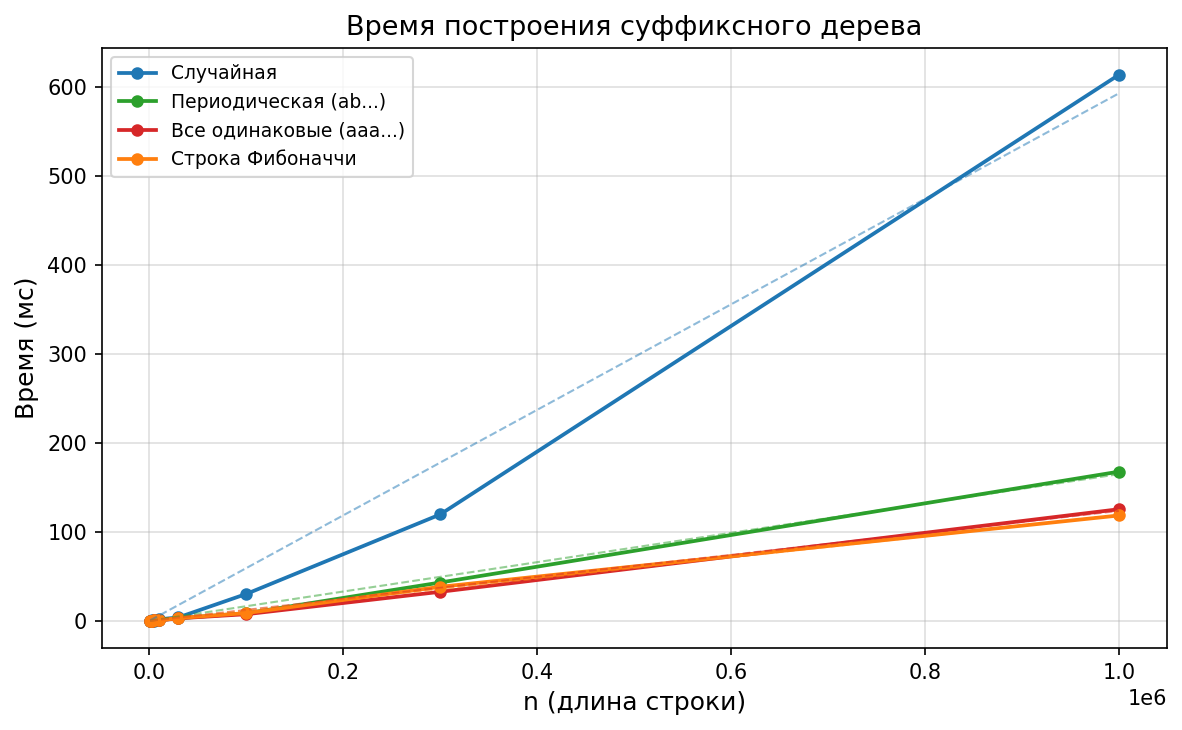
\includegraphics[width=0.9\textwidth]{plot1_time.png}
	\caption{Время построения суффиксного дерева. Пунктир --- подогнанная линия O(n) для каждого типа.}
\end{figure}

Для проверки линейности вычислим отношение
$T(10^6) / T(10^3)$, которое при сложности O(n) должно равняться
$10^6 / 10^3 = 1000$:

\begin{itemize}
	\item однородная: $125536 / 121 \approx 1037$ --- отклонение 3.7\%,
	соответствует O(n);
	\item строка Фибоначчи: $118510 / 116 \approx 1022$ --- отклонение 2.2\%;
	\item периодическая: $167785 / 113 \approx 1485$ --- небольшое
	превышение вследствие накладных расходов при работе с вектором
	на больших объёмах;
	\item случайная: $613980 / 177 \approx 3469$ --- существенное
	превышение. Причина не нарушение асимптотики, а
	\emph{cache miss}: случайные строки порождают хаотичный
	паттерн обращений к памяти, что при $n \sim 10^6$ приводит
	к частым промахам кэша процессора (L2/L3).
	Для детерминированных входов алгоритм ведёт себя строго линейно.
\end{itemize}

\begin{figure}[H]
	\centering
	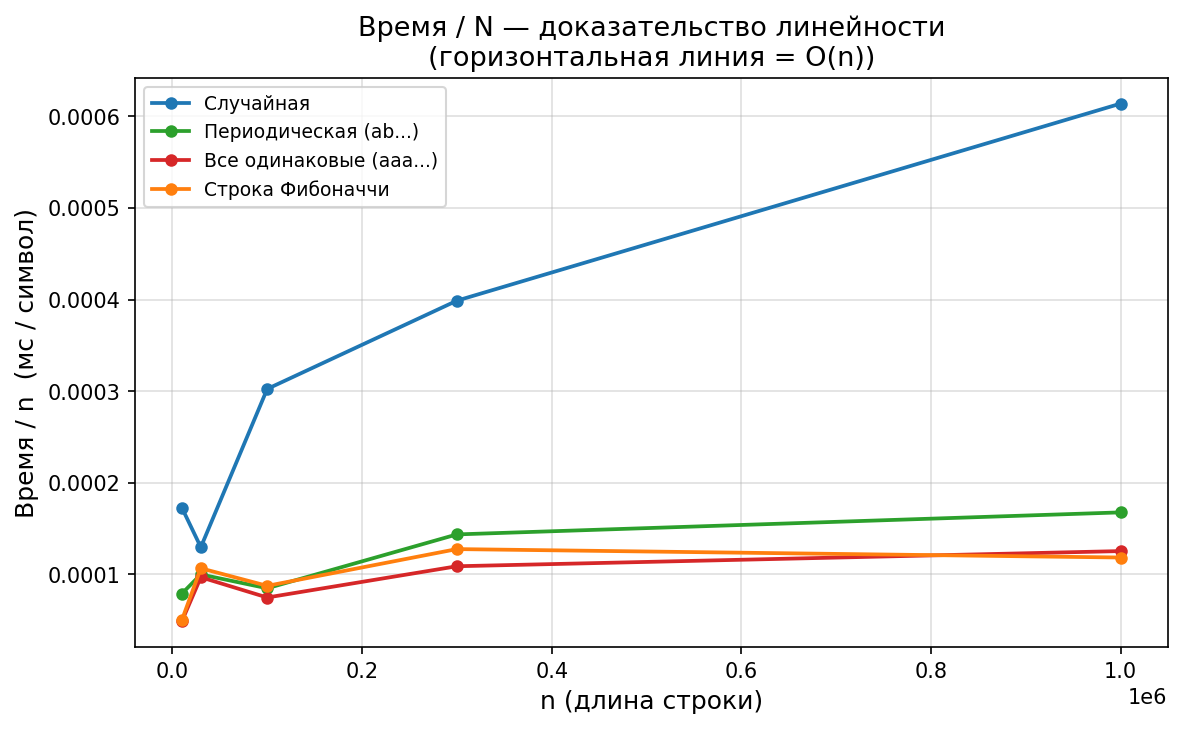
\includegraphics[width=0.9\textwidth]{plot3_ratio.png}
	\caption{Отношение $T(n)/n$. Горизонтальность кривых подтверждает O(n);
		рост кривой случайной строки объясняется эффектом cache miss.}
\end{figure}

Потребление памяти для всех типов строк линейно совпадает
с теоретической оценкой $4n \cdot 120$ байт:
при $n = 10^6$ периодическая, однородная и Фибоначчи
дают ровно $4\,000\,000$ узлов, что точно соответствует верхней
оценке $2(2n+1) - 1 \approx 4n$.

\begin{figure}[H]
	\centering
	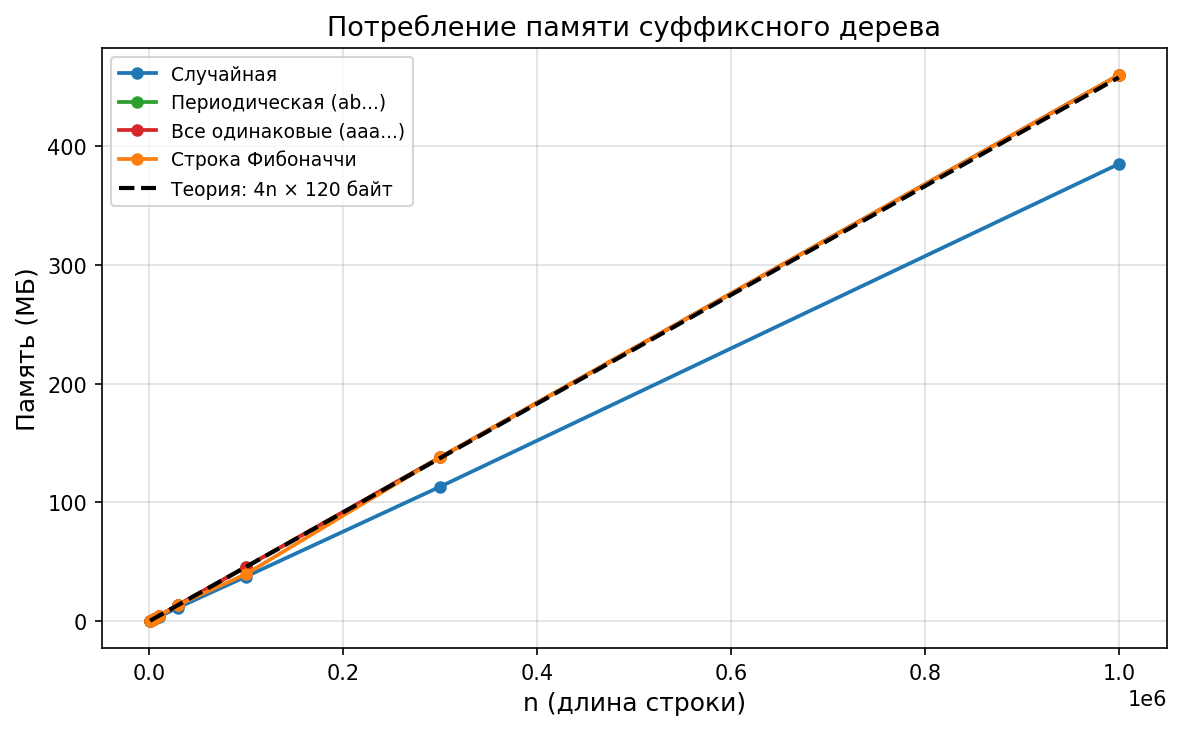
\includegraphics[width=0.9\textwidth]{plot2_memory.png}
	\caption{Потребление памяти. Пунктир --- теоретическая оценка $4n \times 120$ байт.}
\end{figure}


\subsection*{Недочёты}

\begin{itemize}
	\item \textbf{Отсутствие \texttt{nodes.reserve()}.}
	Вектор \texttt{nodes} растёт по стратегии удвоения capacity: при
	каждом переполнении выделяется вдвое больше памяти, чем нужно.
	В момент последнего удвоения фактически выделенная память может
	достигать $2 \times |\text{nodes}| \times 120$ байт. Именно это
	объясняет 966~МБ на тесте~12 при теоретической оценке $\approx 460$~МБ.
	Одна строка \texttt{nodes.reserve(2 * s.size() + 5)} в начале
	\texttt{Build} полностью устранила бы проблему.
	
	\item \textbf{Запас по памяти.}
	На максимальном тесте~12 потребление памяти составило 966~МБ при
	лимите 1~ГБ --- менее 4\% запаса. При незначительном увеличении
	входных данных решение может получить вердикт ML.
	
	\item \textbf{Фиксированный алфавит.}
	Массив \texttt{Children[27]} и функция \texttt{CharIdx} предполагают,
	что входная строка содержит исключительно строчные латинские буквы.
	Символы за пределами диапазона \texttt{a--z} приведут к выходу
	за границы массива. Для обобщения потребовалось бы расширить алфавит
	до 256 символов, что, однако, увеличило бы потребление памяти
	примерно в 9.5~раза.
	
	\item \textbf{\texttt{CharIdx} не проверяет диапазон символов.}
	При любом символе вне \texttt{a--z} и \texttt{SENTINEL} выражение
	\texttt{c - 'a'} даёт индекс вне диапазона \texttt{[0,~26]},
	что приводит к выходу за границы массива \texttt{Children}
	и неопределённому поведению. Программа принимает некорректный
	ввод молча.
	
	\item \textbf{Глобальное состояние алгоритма.}
	Все переменные алгоритма (\texttt{nodes}, \texttt{text},
	\texttt{activeNode}, \texttt{activeEdge} и другие) объявлены
	глобально. Это делает код нереентерабельным: нельзя строить два
	дерева одновременно, сложно писать юнит-тесты. Правильным решением
	была бы инкапсуляция в класс \texttt{TSuffixTree}.
	
	\item \textbf{Посимвольное наращивание строки в \texttt{FindMinRotation}.}
	Строка \texttt{result} формируется операцией \texttt{result += text[i]}
	без предварительного резервирования памяти. При каждой нехватке
	capacity происходит реаллокация и полное копирование, что даёт
	до $O(\log n)$ лишних копирований. Добавление
	\texttt{result.reserve(n)} перед циклом устраняет реаллокации
	и делает формирование результата строго O(n).
	
	\item \textbf{Cache miss на случайных строках.}
	Как показывает тест производительности, на случайных строках
	большого объёма ($n \sim 10^6$) практическое время работы
	растёт быстрее линейного из-за частых промахов кэша процессора.
	Теоретическая сложность O(n) при этом не нарушается, однако
	константный множитель на случайных данных в~5--6~раз выше,
	чем на детерминированных.
\end{itemize}


\subsection*{Выводы}

Суффиксное дерево является универсальной индексной структурой для
строковых задач. Единожды построенное за O(n) по алгоритму Укконена,
оно позволяет эффективно решать широкий класс задач:

\begin{itemize}
	\item поиск подстроки в тексте и нахождение всех позиций
	вхождения за $O(|P| + k)$, где $|P|$ --- длина паттерна,
	$k$ --- число вхождений;
	\item линеаризация циклической строки (данная лабораторная работа)
	--- нахождение лексикографически минимального разреза за O(n);
	\item нахождение наибольшей общей подстроки двух и более строк
	через обобщённое суффиксное дерево;
	\item подсчёт числа различных подстрок строки;
	\item построение суффиксного массива лексикографическим обходом
	листьев дерева.
\end{itemize}

Сложность программирования алгоритма Укконена оценивается как высокая.
Алгоритм оперирует несколькими взаимосвязанными инвариантами
одновременно: активной точкой из трёх переменных
(\texttt{activeNode}, \texttt{activeEdge}, \texttt{activeLen}),
счётчиком \texttt{remaining} и суффиксными ссылками.
Нарушение любого из инвариантов приводит к некорректному дереву,
которое при этом может давать правильные ответы на небольших тестах
и ошибаться только на специально подобранных входах.

Основные трудности при реализации:
выбор структуры хранения дочерних узлов с учётом ограничений
по памяти и времени (от \texttt{std::map} через \texttt{int[128]}
к \texttt{int[27]}), корректная расстановка суффиксных ссылок
при разрезании рёбер, а также обеспечение правильного выбора
символа-стража, который должен быть лексикографически наибольшим,
чтобы алгоритм обхода не уходил по нему раньше времени.


\end{document}

